%%%%%%%%%%%%%%%%%%%%%%%%%%%%%%%%%%%%%%%%%%%%%%%%%%%%%%%%%%%%%%%%%
% !TEX root = interimreport.tex
\clearpage
\chapter{ASCON CRYPTOGRAPHIC ALGORITHM}\label{Chascon}
%%%%%%%%%%%%%%%%%%%%%%%%%%%%%%%%%%%%%%%%%%%%%%%%%%%%%%%%%%%%%%%%%
ASCON (Authenticated Encryption with Associated Data) is a lightweight encryption algorithm that is a family of lightweight authenticated ciphers. ASCON is designed to have both authenticity and confidentiality for transmitted data and it is efficient in terms of both speed and code size. It has a clean and simple design, making it suitable for resource-constrained environments. 
ASCON was designed by Christoph Dobraunig, Maria Eichlseder, Florian Mendel, and Martin Schläffer in 2014. It was proposed as a candidate for the lightweight authenticated encryption competition (CAESAR) in 2014 and was selected as one of the finalists.

\section{ASCON Structure}
Ascon is based on Sponge structure that is shown in Figure \ref{fig:sbox_structure}. ASCON gets an initial input to start and encyrpt the algorithm. The length of the initial input is 320 bits that consists of five 64-bits words. Initial input includes secret key, initial vector and nonce. Secret key is used for the encrypt and decrypt the transmitted information. Information can be read if the key is known thus it must be kept secret. Initial Vector is a random value to start a iterated process. Nonce increases the protection of the cipher against cryptanalysis techniques. 

\begin{figure}
    \centering
    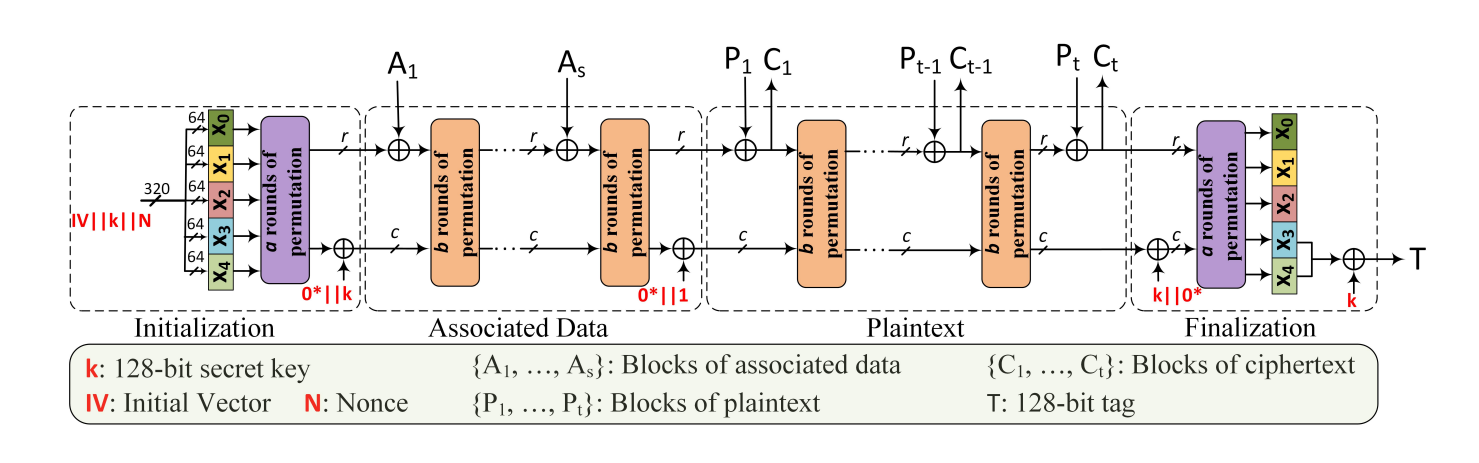
\includegraphics[scale = 0.4]{ascon_sbox/s_box_structure.png}
    \caption{Associated data and plaintext are absorbed into the sponge based structure}
    \label{fig:sbox_structure}
\end{figure}
Concatanated input consists of two parts. The first r bits of the input are the rate bits. The last c = 320 – r bits of the input are called capacity bits. In the initialization stage, “a” rounds of permutaton functions are implemented to concatanated input. After permutation, the last 128 bits of the capacity bits are XORed with 128-bit secret key. 

At the beggining of the associated data stage, rate bits are XORed with the first block of the associated data then “b” rounds of permutation is implemented to the output. This step is repeated with the previous output and the next block of the associated data until all the blocks are covered. Associated data is absorbed into the sponge structure. At the end of the associated stage, capacity bits are XORed with 1’s.

In the Plaintext stage, the plaintext blocks are absorbed into the sponge like the associated stage and the ciphertext blocks are obtained. At the beginning of the finalization stage, secret key is XOR'ed with the first 128 bits of the capacity bits. “a” rounds of permutations are implemented and the last 128 bits of the capacity bits are XORed with the secret key. The output of the finalization stage is called the 128-bit tag. 

\section{Permutation Function of the ASCON Algorithm}


ASCON’s permutation function consists of a nonlinear substition layer and a linear diffusion layer. The substition layer performs a 5-bit S-box. S-box takes five 64-bit concatanated words as input. 64 S-boxes are performed for every bits of the words in a single permutation function. S-box operations are shown in Figure \ref{fig:sbox_operations}. Linear diffusion layer performs the rotations and XOR's shown in Equation \ref{eq:ascon_linear}.

\begin{figure}
    \centering
    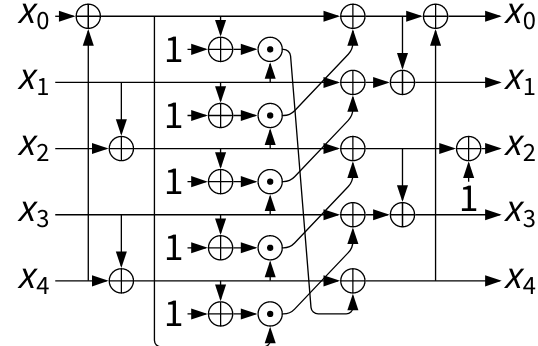
\includegraphics[scale = 0.6]{ascon_sbox/s_box_ascon.png}
    \caption{S-box operations}
    \label{fig:sbox_operations}
\end{figure}

\begin{equation}
\label{eq:ascon_linear}
\begin{aligned}
& x_0 \leftarrow \Sigma_0\left(x_0\right)=x_0 \oplus\left(x_0 \ggg 19\right) \oplus\left(x_0 \ggg 28\right) \\
& x_1 \leftarrow \Sigma_1\left(x_1\right)=x_1 \oplus\left(x_1 \ggg 61\right) \oplus\left(x_1 \ggg 39\right) \\
& x_2 \leftarrow \Sigma_2\left(x_2\right)=x_2 \oplus\left(x_2 \ggg 1\right) \oplus\left(x_2 \ggg 6\right) \\
& x_3 \leftarrow \Sigma_3\left(x_3\right)=x_3 \oplus\left(x_3 \ggg 10\right) \oplus\left(x_3 \ggg 17\right) \\
& x_4 \leftarrow \Sigma_4\left(x_4\right)=x_4 \oplus\left(x_4 \ggg 7\right) \oplus\left(x_4 \ggg 41\right)
\end{aligned}
\end{equation}

